% Copyright (c) 2023 Alexander Bluhm <bluhm@genua.de>
%
% Permission to use, copy, modify, and distribute this software for any
% purpose with or without fee is hereby granted, provided that the above
% copyright notice and this permission notice appear in all copies.
%
% THE SOFTWARE IS PROVIDED "AS IS" AND THE AUTHOR DISCLAIMS ALL WARRANTIES
% WITH REGARD TO THIS SOFTWARE INCLUDING ALL IMPLIED WARRANTIES OF
% MERCHANTABILITY AND FITNESS. IN NO EVENT SHALL THE AUTHOR BE LIABLE FOR
% ANY SPECIAL, DIRECT, INDIRECT, OR CONSEQUENTIAL DAMAGES OR ANY DAMAGES
% WHATSOEVER RESULTING FROM LOSS OF USE, DATA OR PROFITS, WHETHER IN AN
% ACTION OF CONTRACT, NEGLIGENCE OR OTHER TORTIOUS ACTION, ARISING OUT OF
% OR IN CONNECTION WITH THE USE OR PERFORMANCE OF THIS SOFTWARE.

\documentclass[14pt,aspectratio=169]{beamer}
\usetheme{Frankfurt}
\usepackage{tikz}
\usepackage{graphicx}
\usepackage{tipa}
\usepackage{alltt}
\usepackage{xcolor}
\usepackage{upquote}
\usepackage[T1]{fontenc}
\usepackage{textcomp}
\author{Alexander Bluhm}
\title{OpenBSD Security Mitigations}
\institute{genua GmbH\\ \url{bluhm@genua.de}\\ \url{bluhm@openbsd.org}}
\date{September 2023}
\let\Tiny\tiny

\begin{document}

\begin{frame}
\titlepage
\end{frame}

\begin{frame}{Agenda}
\setcounter{tocdepth}{1}
\tableofcontents
\end{frame}

\section{Memory Corruption}

\subsection{Stack Overflow}
\begin{frame}{Stack Overflow}
\begin{itemize}
  \item non executable
  \item random gap, random location
\end{itemize}
\end{frame}

\subsection{Heap Overflow}
\begin{frame}{Heap Overflow}
\begin{itemize}
  \item malloc(3) options
  \item guard page
  \item random chunk order
  \item canaries
\end{itemize}
\end{frame}

\subsection{Heap Use-After-Free}
\begin{frame}{Heap Use-After-Free}
\begin{itemize}
  \item unmap freed
  \item junk at alloc
  \item junk at free
  \item SSH use-after-free
  \item random order
\end{itemize}
\end{frame}

\subsection{Return Oriented Programming}
\begin{frame}{Return Oriented Programming}
\begin{itemize}
  \item map stack
  \item retpoline
  \item fork+exec
  \item signal cookie
  \item arm64 BTI \& Intel IBT endbr64
Random relinking
\end{itemize}
\end{frame}

\subsection{mprotect(2)}
\begin{frame}{mprotect(2)}
\begin{itemize}
  \item W\^{}X
  \item xonly
  \item mimmutable(2)
  \item MAP\_STACK
  \item MAP\_CONCEAL
\end{itemize}
\end{frame}

\subsection{Opportunistic xonly}
\begin{frame}[fragile=singleslide]{Opportunistic xonly}
\begin{verbatim}
  addr = mmap(NULL, 4096, PROT_NONE,
      MAP_PRIVATE | MAP_ANON, -1, 0);
  mprotect(addr, 4096, PROT_READ);
  printf("%p: %08x\n", addr, *(int* )addr);
  mprotect(addr, 4096, PROT_EXEC);
  printf("%p: %08x\n", addr, *(int* )addr);
\end{verbatim}
\begin{verbatim}
  0x73d15433000: 00000000
  0x73d15433000: 00000000
\end{verbatim}
\end{frame}

\subsection{Trap xonly}
\begin{frame}[fragile=singleslide]{Trap xonly}
\begin{verbatim}
  addr = mmap(NULL, 4096, PROT_NONE,
      MAP_PRIVATE | MAP_ANON, -1, 0);
  mprotect(addr, 4096, PROT_READ);
  mprotect(addr, 4096, PROT_EXEC);
  printf("%p: %08x\n", addr, *(int* )addr);
\end{verbatim}
\begin{verbatim}
  Segmentation fault (core dumped)
\end{verbatim}
\end{frame}

\section{Random}

\subsection{Random Everywhere}
\begin{frame}{Random Everywhere}
\begin{itemize}
  \item arc4random(3)
  \item arc4random\_uniform(3)
  \item getentropy(2)
  \item ELF header .openbsd.randomdata
  \item boot /etc/random.seed
\end{itemize}
\end{frame}

\subsection{Address Space Layout Randomization}
\begin{frame}{Address Space Layout Randomization}
\begin{enumerate}
  \item shared library mapping
  \item heap mmap(2)
  \item stack gap
  \item PIE program text
  \item relink libc
  \item relink sshd(8)
\end{enumerate}
\end{frame}

\subsection{Address Space Layout}
\begin{frame}{Address Space Layout}
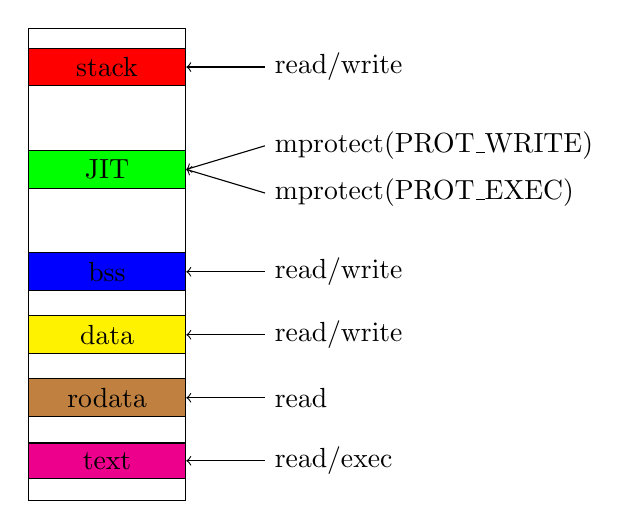
\begin{tikzpicture}
\path
    (0,0) node [draw,below,minimum width=2cm,minimum height=6cm] (proc) {}
    +(0,-0.5) node [draw,minimum width=2cm,fill=red] (stack) {stack}
    +(0,-1.8) node [draw,minimum width=2cm,fill=green] (jit) {JIT}
    +(0,-3.1) node [draw,minimum width=2cm,fill=blue] (bss) {bss}
    +(0,-3.9) node [draw,minimum width=2cm,fill=yellow] (data) {data}
    +(0,-4.7) node [draw,minimum width=2cm,fill=brown] (rodata) {rodata}
    +(0,-5.5) node [draw,minimum width=2cm,fill=magenta] (text) {text};
\draw (stack.east) [<-] -- +(1,0) node [anchor=west] {read/write};
\draw (jit.east) +(1,0) node [anchor=south west] (mwrite)
    {mprotect(PROT\_WRITE)} (mwrite.west) [->] -- (jit.east);
\draw (jit.east) +(1,0) node [anchor=north west] (mexec)
    {mprotect(PROT\_EXEC)} (mexec.west) [->] -- (jit.east);
\draw (bss.east) [<-] -- +(1,0) node [anchor=west] {read/write};
\draw (data.east) [<-] -- +(1,0) node [anchor=west] {read/write};
\draw (rodata.east) [<-] -- +(1,0) node [anchor=west] {read};
\draw (text.east) [<-] -- +(1,0) node [anchor=west] {read/exec};
\end{tikzpicture}
\end{frame}

\subsection{Special Protection}
\begin{frame}{Special Protection}
\end{frame}

\subsection{Kernel Exec}
\begin{frame}{Kernel Exec}
\begin{itemize}
  \item check argc > 0
  \item random stack
  \item random signal cookie
  \item exec pledge
  \item setuid open stdin, stdout, stderr
\end{itemize}
\end{frame}

\subsection{Dynamic Loader}
\begin{frame}{Dynamic Loader}
\begin{itemize}
  \item init random getentropy(2)
  \item fix permissions mimmutable(2)
  \item random layout mmap(2)
  \item syscall area msyscall(2)
  \item exec area pinsyscall(2)
  \item lazy-binding kbind(2)
\end{itemize}
\end{frame}

\subsection{Others}
\begin{frame}{Others}
\begin{itemize}
  \item exec options
  \item xonly
  \item reallocarray(3)
  \item explicit\_bzero(3)
  \item sigreturn(2)
  \item mount options
  \item printf(3) \%n
  \item fork+exec
  \item otto malloc in practice
  \item secure by default and enforced
  \item ssh attack -> process trace, libc malloc reuse
  \item ssh agent -> executable stack enforced
\end{itemize}
\end{frame}

\subsection{SSH Agent Library Exploit}
\begin{frame}{SSH Agent Library Exploit}
dlopen(3) 4 libraries:
\begin{itemize}
  \item ELF header executable stack 
  \item init signal handler SIGSEGV
  \item ELF flag NODELETE
  \item on load segmentation fault
\end{itemize}
\end{frame}

\subsection{Default and Force}
\begin{frame}{Default and Force}
\begin{itemize}
  \item control: kernel, libc, base
  \item adapt: ports
  \item last resort: program and mount flags
\end{itemize}
\end{frame}


\section{Not yet}
\begin{frame}{Not Yet}
\begin{itemize}
  \item ARM pointer authentication
  \item shadow stack
\end{itemize}
\end{frame}

\subsection{Questions}
\begin{frame}{Questions}
\begin{center}
\begin{tikzpicture}
\draw [font=\Huge] node {?};
\end{tikzpicture}
\end{center}
\end{frame}

\end{document}
